\chapter{Computer Vision}
The computer vision part is the image processing part of the project. Here the machine differentiates the different \lego bricks and their individual colours. Furthermore their pixel position is found to be converted to world coordinates later in the program.
This is done to let the robot use the knowledge of the different colours to automatically assemble the figures with the right coloured bricks.
To find the bricks in the picture, several steps are made to differentiate the colours:

\begin{itemize}
	\item Format conversion
	\item Background subtraction
	\item Colour thresholding
	\item Noise removal
	\item BLOB analysis
	\item Feature extraction
\end{itemize}

The original picture processed is shown in \autoref{fig:orig_pic}.

\begin{figure}
	\centering
	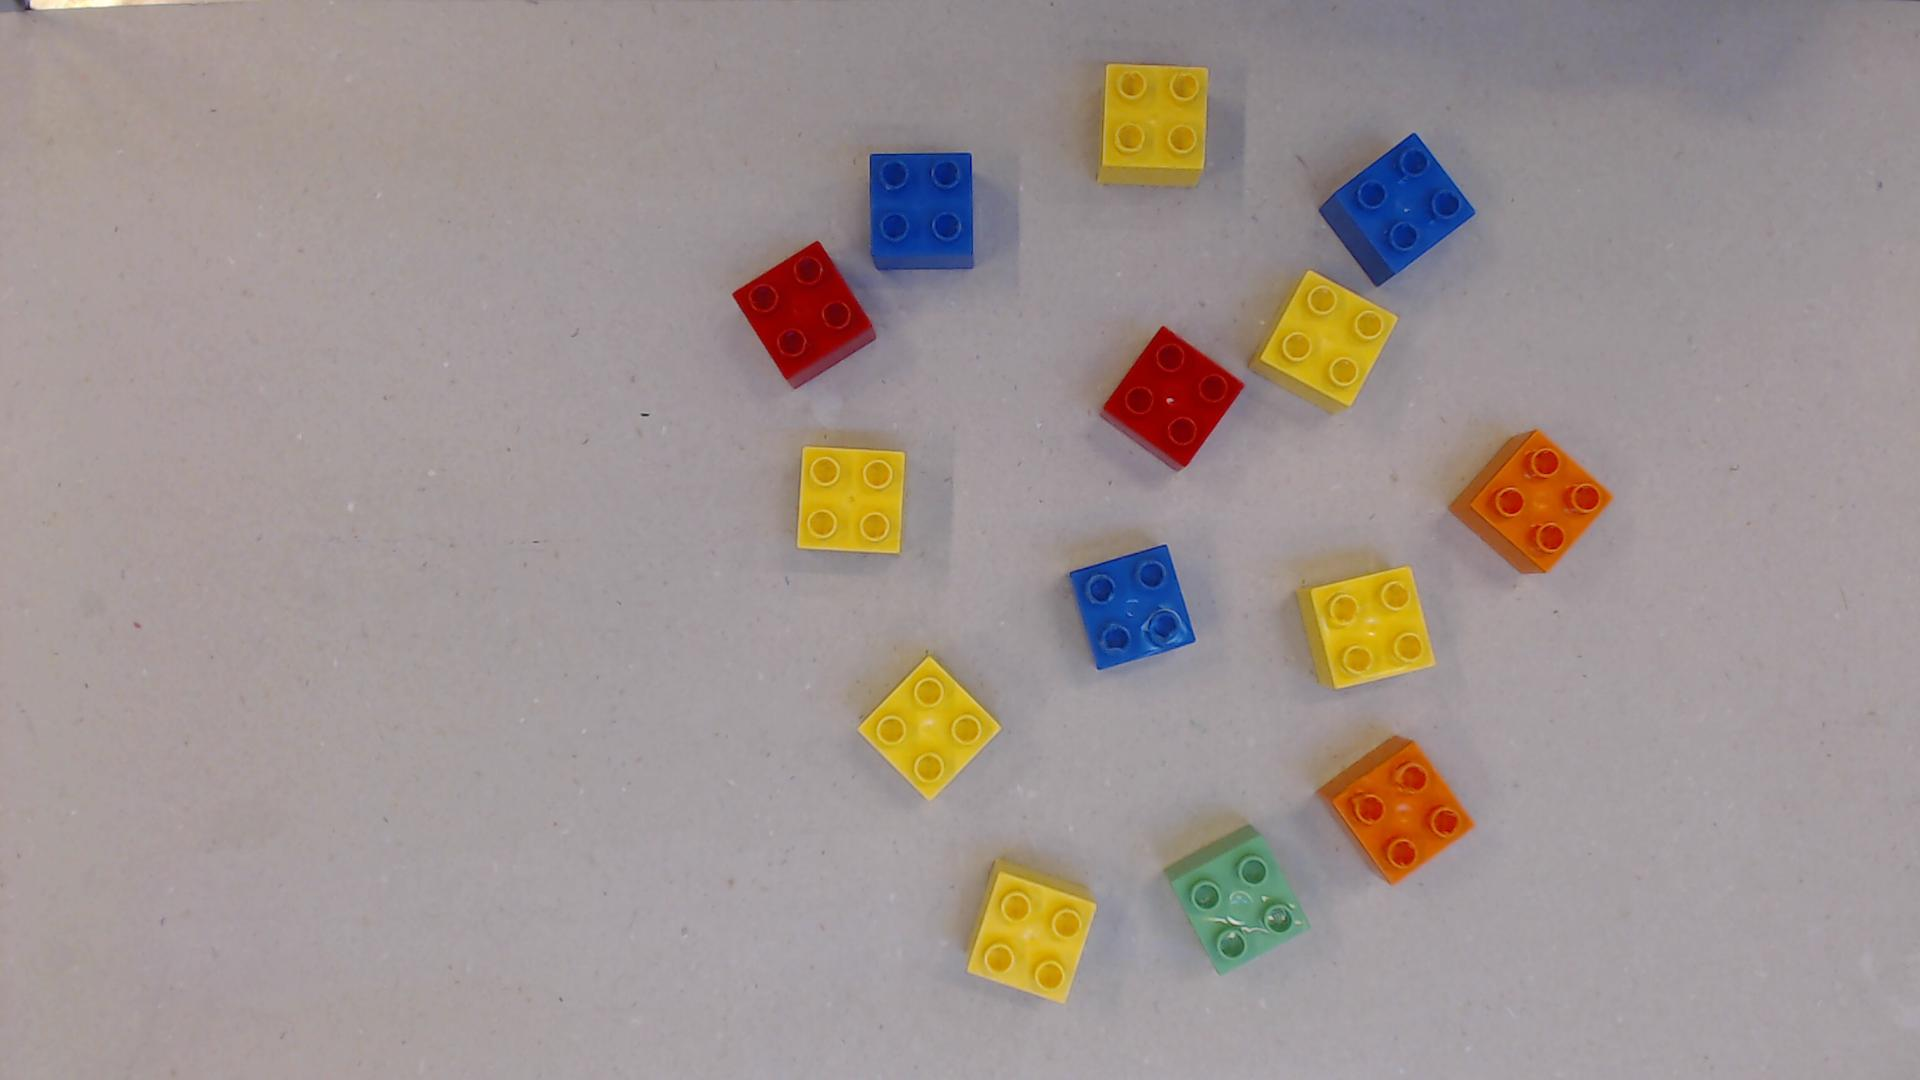
\includegraphics[width=0.69\textwidth]{figures/orig_pic.jpg}
	\caption{Original picture taken by the webcam attached to the robot.}
	\label{fig:orig_pic}
\end{figure}

\section{Format Conversion}
The original picture taken by the webcam is in RGB and is converted to a chromaticity image. This is done using \autoref{eq:rgb_to_rgi}:

\begin{equation}\label{eq:rgb_to_rgi}
	r=\frac{R}{R+G+B}, ~g=\frac{G}{R+G+B}, ~I=\frac{R+G+B}{3}
\end{equation}

Chromaticity is given from the chromaticity plane. This is shown in \autoref{fig:chrom_plane}. This is done since the colours are being normalised to avoid influence by illumination. Then the colour description is supplemented by an intensity as calculated in \autoref{eq:rgb_to_rgi}. This will be referred to as RGI and the conversion is RGB to RGI.


\begin{figure}[H]
	\centering
	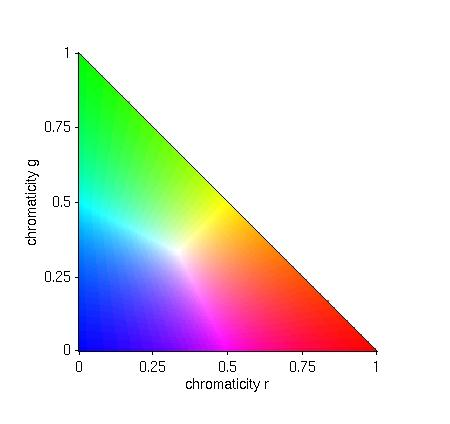
\includegraphics[width=0.7\textwidth]{figures/chrom_plane}
	\caption{Chromaticity plane}
	\label{fig:chrom_plane}
\end{figure}

\section{Background Subtraction}

\section{Colour Thresholding}

\section{Noise Removal}

\section{BLOB Analysis}

\section{Feature Extraction}
